\chapter{Alignment, Authorization, and Constrained Autonomy}\label{ch:C29}
OpenAI Agents Python v0.24.0's October change to defer automatic compaction during pending approvals exposes an alignment problem with a concrete runtime boundary~\cite{executionrelease02}. A review request, the evidence it refers to, and the proposed effect must remain interpretable until a decision is applied. The release note establishes an implementation change, not universal approval correctness. Combined with Progent's distinction between policy narrowing and expansion, it motivates treating objectives, evidence, authority, and dispatched effects as separate versioned commitments~\cite{corpus250411703}.

Alignment concerns how system behavior relates to intended objectives, preferences and constraints. Authority concerns who may define or change those objectives and which effects the system may cause. The distinction is essential for agents. A model can correctly infer a user's preference while lacking permission to act on it; an application can enforce permissions while optimizing an inappropriate proxy. Reliable autonomy requires both a useful policy and a current, enforceable account of authority.

This chapter connects training objectives to operational control, human review, privacy, memory and deployment decisions. It treats approvals, monitors and evaluators as fallible components. No finite evaluation establishes universal alignment, and no role label or persistent identity establishes that a system understands organizational intent. The practical question is which constraints can be enforced, which judgments can be measured, and which uncertainties remain material to deployment.

\section{Objectives proxies and constrained policies}\label{sec:C29:objectives}
A sequential objective can maximize expected discounted task reward, but the reward is a representation of intent rather than intent itself. Outcome labels may omit constraints, reward models may favor presentation, and benchmark graders may accept shortcuts. An agent optimized against such feedback can improve the measured objective while worsening the underlying task. This is a specification and evaluation problem as well as a learning problem.

Let $r_t$ denote task reward and $c_{j,t}$ a cost or constraint-violation signal. A constrained formulation is
\begin{equation}
 \max_{\pi}\;\mathbb E_\pi\sum_t\gamma^t r_t,
 \qquad
 \mathbb E_\pi\sum_t\gamma^t c_{j,t}\leq d_j.
\end{equation}
For this infinite-horizon expression, $t\in\mathbb N_0$, $\gamma\in[0,1)$, $j\in\{1,\ldots,J\}$ indexes a finite set of constraints, $d_j\geq0$ are thresholds, and rewards and nonnegative costs are bounded. A finite-horizon study instead truncates both sums at its declared stopping time. The constraints remain meaningful only if the signals and thresholds represent the desired properties. A positive expected-cost budget can permit rare severe violations. An exactly zero expectation of nonnegative costs would exclude positive costs almost surely at positively weighted times under the modeled law, but a finite sample of zero observed costs does not establish that premise; $\gamma=0$ does not constrain later times at all. An authorization requirement may instead demand that every dispatched action belong to the current allowed set. That property should be enforced at the effect boundary rather than traded against reward through an arbitrary finite penalty.

Reward shaping and refusal training can reduce undesirable proposals, but they do not establish complete mediation. A model can encounter a novel representation or be placed inside a harness that grants broader tools. Conversely, a runtime policy can block unauthorized effects even when the model proposes them. Evaluate proposal behavior and executed behavior separately so a successful control layer is visible without misrepresenting the model's alignment.

Preference learning introduces population and context questions. Whose preferences are represented, under what task, and with which exceptions? A user preference stored months earlier may conflict with a current instruction or an organizational rule. Treating all preferences as timeless facts creates predictable errors. A policy should represent scope, provenance and update authority rather than simply weight the most frequently retrieved statement.

The practical implication is to separate hard constraints, uncertain judgments and optimization objectives. Hard constraints require application-enforced checks where possible. Uncertain judgments require calibrated evidence and review. Objectives guide useful behavior within those boundaries. Collapsing the three into a single textual instruction or scalar reward makes it harder to identify which mechanism failed.


\section{Instruction hierarchy and authority-bearing records}\label{sec:C29:hierarchy}
An instruction hierarchy organizes competing directives by source and scope. Its implementation must distinguish an authorized user request, application policy, tool metadata, external evidence and model-generated plans. Text that describes a rule is not automatically an authoritative rule. A retrieved document can quote an instruction without being allowed to change the agent's task or permissions.

Authority-bearing records should identify the principal, action scope, affected objects, validity interval and policy epoch. An approval to edit a draft does not authorize sending it to an external recipient. Approval of one argument set does not authorize a later modified request. The runtime should bind approval to the exact operation or to a clearly specified capability envelope, then revalidate at dispatch.

Historical authority and current authority differ. Session logs preserve what was requested or granted earlier; the authorization service determines what is allowed now. Restoring a checkpoint should not resurrect expired or revoked grants. This separation can be enforced structurally even when the model's context contains the old instruction. The tool boundary should consult current authority independently of the model's interpretation.

The same principle applies to delegation. A manager may delegate reasoning without delegating every tool capability or every source document. Workers should receive the minimum context and authority needed for their subtask. A handoff must preserve restrictions and identify who remains responsible for the final effect. Internal agent messages should not become a privileged channel for promoting untrusted content.

Instruction-hierarchy evaluation should include conflicting but plausible directives, ambiguous provenance, changed permissions and resumed sessions. Measure whether the system identifies the governing source, requests clarification when necessary, and prevents unauthorized effects. A benchmark consisting only of obvious malicious strings tests a narrower capability. It cannot establish correct authority reasoning in ordinary multi-party workflows.


\section{Constitutional and preference-based alignment}\label{sec:C29:training}
Post-training can shape how a model interprets requests, critiques outputs and handles uncertain or harmful tasks. The 2022 Constitutional AI procedure provides a foundational example of using stated principles and AI feedback in training~\cite{bai2022constitutional}. The contribution concerns a training procedure and its evaluated behaviors. It does not establish that a deployed agent automatically follows every organizational policy or that a principle list resolves all contextual conflicts.

Preference optimization depends on the data-generation and judging process. If preferred responses are selected for fluency, completeness or agreement, a model can learn to present unsupported confidence. If refusals are rewarded too broadly, useful benign tasks may be blocked. Evaluate both harmful compliance and benign-task retention under the actual tool environment. A model-only conversation study and an effectful agent deployment have different action spaces.

AI-generated critique is useful feedback but can share the original model's blind spots. A critic may miss a constraint, infer a requirement not present in the task, or agree with a misleading rationale. Independent executable evidence can complement critique where available. For semantic or ethical judgments without a complete oracle, report the adjudication procedure and disagreement rather than treating the critic's role as proof of correctness.

Training can also change memory interpretation. A new policy may give stronger weight to persistent preferences or be more skeptical of retrieved instructions. Existing skill banks and summaries were written under earlier behavior. An alignment update can therefore improve one task family while producing compatibility regressions elsewhere. Model migration tests should include old memory, conflicting updates and changed authority, not only fresh prompts.

The relevant causal comparison holds the harness and information budget fixed while varying the trained policy, then separately tests interactions with context and memory mechanisms. If a post-training method changes output format or tool-call tendencies, the parser and evaluator may need compatible configuration. Report those changes rather than attribute every difference to an abstract quality called alignment.

\subsection{Automated safety adaptation and independent confirmation}\label{sec:C29:automatedalignment2026}
A3's March 2026 report supplies a concrete automated safety-finetuning loop: generate hypotheses around a failure, construct harmful and benign counterparts, tune LoRA and data mixtures, and retain experiment results for subsequent choices~\cite{zhang2026a3}. Its reported experiments primarily concern Qwen-2.5-7B Instruct, with one additional Llama setting, rather than the October frontier-model population. This is evidence for targeted adaptation under the tested feedback loop, not a result that arbitrary safety properties can be repaired automatically or transferred without regression.

The code reveals a material evaluation boundary. In the inspected \path{IterativeLoRASFTAgent}, \path{select_hyperparameters} consumes previous results; the selection prompt explicitly prioritizes constraints on both validation and OOD performance. The experiment log written by \path{update_experiment_log} includes OOD aggregate and per-hypothesis outcomes~\cite{a32026code}. Therefore hypothesis-disjoint OOD data are not equivalent to an untouched final assessment when their performance can guide later iterations. This does not imply that OOD examples were inserted into training; the selection prompt separately restricts training weights to training hypotheses. The issue is adaptive evaluation feedback, which changes the independence claim even when example-level splits remain intact.

Let $D_{\mathrm{dev}}$, $D_{\mathrm{shift}}$ and $D_{\mathrm{confirm}}$ denote development, shift-diagnostic and final-confirmation populations. An optimizer may legitimately use the first two to choose a candidate, but confirmation requires the selected artifact and procedure to be fixed before revealing the third population's outcomes. Repeated shift diagnostics help discover failure modes; they cease to be untouched evidence as soon as they influence selection. Record every query and rejected candidate, include benign refusal and capability regressions, and repeat with independent hypothesis generators and judges. The update should then be tested with old memory, pending approvals and existing tool schemas, because targeted output improvements do not establish compatibility with a stateful deployment.

Diffuse AI Control supplies a complementary 2026 warning about optimizing weak scorers on difficult-to-grade research proposals~\cite{terekhov2026diffuse}. Its red team searches for proposals that a weak scorer rates highly while a stronger information-privileged proxy rates poorly. The stronger scorer is itself a proxy, and the improved blue-team prompts are found using access to that proxy. The result therefore demonstrates a configured oversight failure and a proof-of-concept mitigation under privileged search, rather than a generally available guarantee against research sabotage. The appropriate synthesis is to improve the feedback channel, isolate final assessment and enforce authority boundaries; automating the optimizer does not remove the need to validate the criterion it optimizes.

\section{Human review and the semantics of approval}\label{sec:C29:review}
Human review can supply judgment, authority or both. A reviewer may assess whether an artifact is technically sound, while a different principal authorizes publication. Combining these decisions into one button can create ambiguity. The interface should state what is being reviewed, which effect is being authorized, and what evidence remains uncertain. Approval should not be inferred from silence, elapsed time or a historical response to another request.

Review is a limited resource. Long agent-generated explanations can overload the reviewer or hide decisive facts among plausible detail. A useful review surface presents the exact proposed effect, artifact identity, scope change, evidence, failed checks and unresolved consequences. It should distinguish facts derived from execution records from claims generated by the model. This supports informed intervention without pretending that a human inspects every token.

The October Agents SDK release notes explicitly defer automatic compaction while approvals are pending~\cite{executionrelease02}. This is a concrete interaction between context management and authority: changing the context during an unresolved approval can remove or alter the evidence needed to interpret it. The fix is version-specific evidence about one boundary, not a universal solution to approval correctness. Applications must still bind the approval to the action and current policy epoch.

A review experiment can seed defects and vary the presentation of evidence under a fixed time budget. Measure detection, false rejection, decision time, and whether approved actions match what reviewers believed they approved. Also test changes after approval: if the artifact digest or arguments differ at dispatch, the old approval should fail validation. This is a mechanical invariant independent of the reviewer's technical skill.

The check must also have a declared commitment point. Write a grant as $g=(p_g,\mathcal C_g,\alpha_g,t_g)$, binding principal, approved operation envelope, policy epoch, and expiry. For operation $a$ and current principal $p$, a conservative commit-time admission predicate is
\begin{equation}
 \mathbf1\{p=p_g,\ a\in\mathcal C_g\cap F_{\alpha(t)}(t),\
 \alpha(t)=\alpha_g,\ t\leq t_g\}.
\end{equation}
Here an operation includes its arguments, object versions and purpose; $F_{\alpha(t)}(t)$ is the current authoritative feasible set. Requiring epoch equality intentionally invalidates old grants after any governing policy change; a service may instead support a formally specified revalidation rule. Checking this predicate before an unrelated remote write leaves a race between check and use. Enforcement needs a version-conditional or otherwise atomic service contract at the relevant effect boundary. If the service exposes no such primitive, report the residual race and reconciliation behavior rather than claim that an earlier approval proves current authorization. Cancellation cannot retract an effect already committed under the service's own ordering rules.

Escalation policies should distinguish missing preference, missing authority and missing evidence. A user can clarify desired behavior but may not have permission to override an organizational restriction. An administrator can grant a capability without establishing that the proposed action is technically correct. The system should route the question to the appropriate role rather than asking an undifferentiated human oracle to resolve every uncertainty.


\section{Privacy purpose and the lifecycle of memory}\label{sec:C29:privacy}
Privacy depends on collection, use, sharing, retention and deletion, not only on whether storage is encrypted. An agent may retrieve a permitted document for one purpose and later reuse its summary in another context where that use is inappropriate. A memory record therefore needs subject, source, purpose, audience, validity and retention metadata in addition to content. These fields influence both retrieval and action authorization.

Purpose limitation is difficult to infer from natural language alone. A broad request to help with a project does not necessarily authorize exporting every related document. Application logic should define the available capability envelope, and the agent should request additional authority only when the task requires it. The request should identify the specific effect and evidence, not seek a blanket expansion that persists indefinitely.

Deletion has several meanings. Logical exclusion prevents future retrieval; physical removal deletes stored bytes; derivative invalidation addresses summaries, embeddings and skills; parameter unlearning concerns information absorbed into model weights. Completing one does not establish the others. A system should accurately report which action occurred and which copies or retention obligations remain. External disclosure cannot generally be undone by deleting the local source.

Shared memory raises multi-user conflicts. A procedure learned from one user's private task may be useful to another, but utility does not grant permission to share it. Abstraction can still reveal sensitive details or encode privileged assumptions. A promotion process should check whether the generalized skill contains source-specific information and whether its reuse is authorized. Evaluation should include cross-user leakage and benign transfer rather than reward sharing alone.

Privacy-aware traces require a similar balance. Detailed records support auditing and reproducibility but can expose the very content the system should protect. Separate access-controlled raw evidence from redacted operational metadata, define retention, and preserve stable identities so authorized auditors can join records. If redaction removes decisive evidence from public artifacts, state the resulting verification limit rather than imply full independent reproducibility.


\section{Operational constraints and residual risk}\label{sec:C29:operations}
Operational alignment includes budgets, deadlines, service objectives and recovery authority. A model can pursue a task too aggressively, continuing to consume resources after progress becomes unlikely or repeating actions after cancellation. Hard budget enforcement should reside outside the policy. The policy can allocate resources within the envelope, but it should not be able to redefine the envelope through persuasive narration.

Risk-sensitive objectives may emphasize tail losses rather than average success. A deployment can tolerate occasional formatting errors while requiring much stronger control of disclosure or destructive actions. Expected utility alone can hide that asymmetry. Constraints, review gates and effect-specific authority provide a more transparent mechanism than one global confidence threshold. Their effectiveness still needs empirical validation and explicit assumptions.

Monitoring detects drift in both behavior and environment. Changes in tool schemas, model versions, user populations or memory contents can invalidate earlier evaluations. A monitor should identify the version and state associated with an alert, support containment, and preserve evidence for diagnosis. A conceptual AgentOps framework organizes observation and automation needs~\cite{corpus250711277}; operational benefit requires implementation and measured workload evidence beyond the framework's taxonomy.

Rollback must include compatible model, prompt, harness, tool and memory versions. Restoring only model weights can leave skills written for a later policy or an index built with another representation. External effects require reconciliation and may remain irreversible. The authority to initiate rollback should itself be specified, especially when several organizational owners control different components.

Incident learning should avoid feeding unverified explanations directly into persistent memory. A model's account of why a failure occurred is a hypothesis. Validate it against logs, environment state and counterfactual tests before promoting it into a reusable rule. Otherwise an operational failure can become a misleading skill that causes future regressions. This is the same evidence-promotion problem encountered in research agents, now applied to deployment governance.


\section{Evaluation of authority and aligned behavior}\label{sec:C29:evaluation}
An authority evaluation needs tasks where the desired outcome and permitted action set are explicit. Include legitimate completion, conflicting instructions, expired grants, revoked access, ambiguous requests, delegated workers and pending effects. The evaluator should observe actual tool dispatch and environment changes, not only the final answer. A policy that verbally refuses but still causes an unauthorized effect has failed the operational constraint.

Separate model judgment from enforcement. Measure whether the model proposes appropriate actions, whether the runtime blocks disallowed ones, and whether useful work completes. This decomposition identifies complementary improvements. Better model behavior can reduce review and rejection load; stronger enforcement can contain residual mistakes. A combined score without these components cannot explain which layer supplies reliability.

Human-AI collaboration frameworks can clarify role expectations and degrees of agency~\cite{corpus250814825}. Their conceptual categories should not be treated as empirical proof of trust, shared intentionality or appropriate delegation. Evaluate the actual workflow: what the human understands, what the agent can change, and whether authority remains legible after interruptions and handoffs. Anthropomorphic language can otherwise conceal concrete responsibility gaps.

The statistical design should preserve user and organization clusters, because policies and preferences are shared within them. Repeated prompts against one policy do not establish cross-organization generalization. Include heterogeneous task families and report failures by authority type and consequence. Adaptive tests should search for boundary violations under declared budgets while benign tests measure overblocking and review burden.

The conclusion should be a bounded operational claim. A system can demonstrate useful behavior under specified objectives, constraints, principals and environments. It cannot infer unrestricted alignment from a high benchmark average, a constitutional prompt or a human-review stage. The scientific task is to make those conditions explicit, measure where they hold, and retain evidence about where they fail.

\section{A governed model-and-harness update}\label{sec:C29:updatecase}
Consider an agent authorized to improve an internal research workflow. It can propose prompts, context policies, tool adapters and reusable skills, then evaluate candidates on a development set. It cannot change the final assessment set, grant itself new data access, or deploy a candidate without the designated release authority. The desired outcome is better verified research quality within a resource envelope, not merely a larger development score. This case brings alignment, scientific validity and operational authority into the same concrete transition.

The first boundary is between proposal and commitment. Candidate changes are stored in an isolated workspace with a manifest identifying model parameters, harness revision, prompts, tools, memory schema and evaluator configuration. Running an experiment does not authorize promotion. A model can describe a candidate as successful, but the release record must refer to the exact artifact and evidence reviewed. If the candidate changes after review, the old decision no longer applies automatically.

The second boundary is between development and assessment. The agent may inspect development failures to form hypotheses, but an untouched assessment set must remain outside its ordinary tools and memory. If it sees the assessment outcomes repeatedly and modifies the workflow accordingly, that set becomes an optimization resource. This remains true when only prompts or skills change. Frozen model weights do not preserve statistical independence of the final evaluation.

A scalar reward cannot by itself guarantee this separation. Suppose the agent's objective is task benefit minus a penalty $\lambda$ for a prohibited evaluation change. If a candidate can obtain benefit greater than the finite penalty, the penalized objective can prefer the prohibited change. Even if the intended benefit is bounded, the implementation may mismeasure it or expose an exploitable proxy. A hard application constraint on evaluator modification is therefore a different mechanism from discouraging such modification through reward.

This argument does not imply that all behavioral constraints must be expressed as low-level rules. Many aspects of research quality, honesty and relevance require judgment. It implies that constraints with clear effect boundaries should be enforced there, while uncertain semantic judgments are evaluated with evidence and review. Treating both as one preference score obscures whether a failure arose from missing authority checks or from an inadequate quality model.

The third boundary is memory compatibility. A candidate harness may interpret existing skills differently, or its context constructor may omit provenance that the previous policy relied on. Evaluating only fresh tasks from empty memory can miss these regressions. The release test should include saved longitudinal states, contradictory evidence, old procedural records and permission changes. Passing a schema migration establishes representational compatibility, while behavior under the migrated state requires separate tests.

Table~\ref{tab:C29:release} organizes the commitments. Each transition has an owner and an evidence obligation. The table is a governance design rather than a claim that any named product implements the entire process.
\begingroup\setlength{\tabcolsep}{3pt}\small
\begin{longtable}{L{24mm}L{39mm}L{45mm}}
\caption{Authority and evidence in a controlled agent update.}\label{tab:C29:release}\\
\toprule Transition & Authority boundary & Evidence obligation \\
\midrule\endfirsthead
\toprule Transition & Authority boundary & Evidence obligation \\
\midrule\endhead
Propose candidate & Agent may edit only declared development components. & Immutable diff and manifest identify every changed dependency. \\
Run development & Experiment budget and data grants remain external controls. & Complete outcomes include failures, costs and rejected candidates. \\
Assess candidate & Final evaluator and holdout remain independently controlled. & Verdict binds to the fixed candidate and declared test population. \\
Review release & Technical review and deployment authority are identified separately. & Reviewer sees regressions, unresolved evidence and scope changes. \\
Commit release & Approval binds to artifact digest and current policy epoch. & Dispatch checks that the reviewed object is still the deployed object. \\
Monitor and revert & Operational owner can contain or restore within a declared envelope. & Traces preserve affected tasks, state versions and residual effects. \\
\bottomrule\end{longtable}
\endgroup

An interruption can expose a subtle approval failure. The agent prepares a release, obtains a pending review request, compacts its history, and later resumes after the reviewer responds. If compaction removed the exact candidate or scope, the response can be applied to the wrong operation. The release-specific SDK behavior discussed earlier provides evidence that pending approvals and context transformations interact in real implementations. The general invariant is stronger: approval identity and scope must be stored outside a lossy summary and revalidated against the current candidate.

The reviewer should not receive only the agent's preferred narrative. Present the full candidate manifest, comparison protocol, aggregate and stratified outcomes, negative results, changed permissions, and untested conditions. A model-generated recommendation can accompany these records but should be labeled as interpretation. This reduces the chance that persuasive prose becomes a substitute for evidence. It also makes disagreement between technical review and deployment authorization explicit rather than forcing both into one approval state.

The proposed experiment injects a candidate change after approval, an evaluator-version mismatch, a stale skill bank, a revoked data grant and a delayed review response. Compare text-only approval tracking with digest-bound records and current-epoch validation. Measure unauthorized promotion, stale-evidence acceptance, valid-release completion, review burden and recovery cost. The experiment should include benign updates so a system that blocks every release does not appear successful merely because no unsafe update occurs.

Failure attribution should follow the transition chain. If the assessor read the wrong artifact, the problem is evidence identity. If it read the correct artifact but missed a regression, the problem is evaluator coverage or judgment. If the release service ignored an expired approval, the problem is enforcement. If the agent optimized the wrong outcome while obeying all permissions, the objective or specification needs revision. These diagnoses require different interventions and should not collapse into an undifferentiated alignment failure.

The case also exposes responsibility for residual uncertainty. A release authority can decide that available evidence is sufficient for a bounded deployment, but that decision does not convert unknown behavior into known safety. Monitoring and rollback reduce some consequences while leaving irreversible effects and unobserved regressions possible. The assurance record should retain those limitations and identify which new observation would trigger containment or reevaluation.

Useful autonomy is therefore a relationship among a policy, its authorized action space, evidence-producing evaluators and accountable operators. Training improves the policy's choices within that relationship. Context and memory preserve the information those choices require. Runtime controls prevent stale or unauthorized commitments. Scientific evaluation measures the resulting behavior under declared conditions. The research goal is to strengthen each connection while resisting the temptation to let success at one layer stand in for assurance about the others.

A release record should also identify the scope of any claimed guarantee. Passing a fixed regression suite supports behavior on that suite; a proof of a permission invariant supports the modeled action boundary; a reviewer decision records an authorized judgment. These records can coexist without being interchangeable. The release service can require all three for a particular effect while still preserving their separate failure modes. If one dependency changes, invalidate only the claims whose premises changed and rerun their associated checks. This dependency-aware assurance is more scalable than repeating every test after every edit, and more defensible than assuming that an unchanged product name implies unchanged behavior.


The approval-to-commit gap in Figure~\ref{fig:C29:overview} persists unless the service binds validation to commitment.
\begin{figure}[!htbp]
\centering
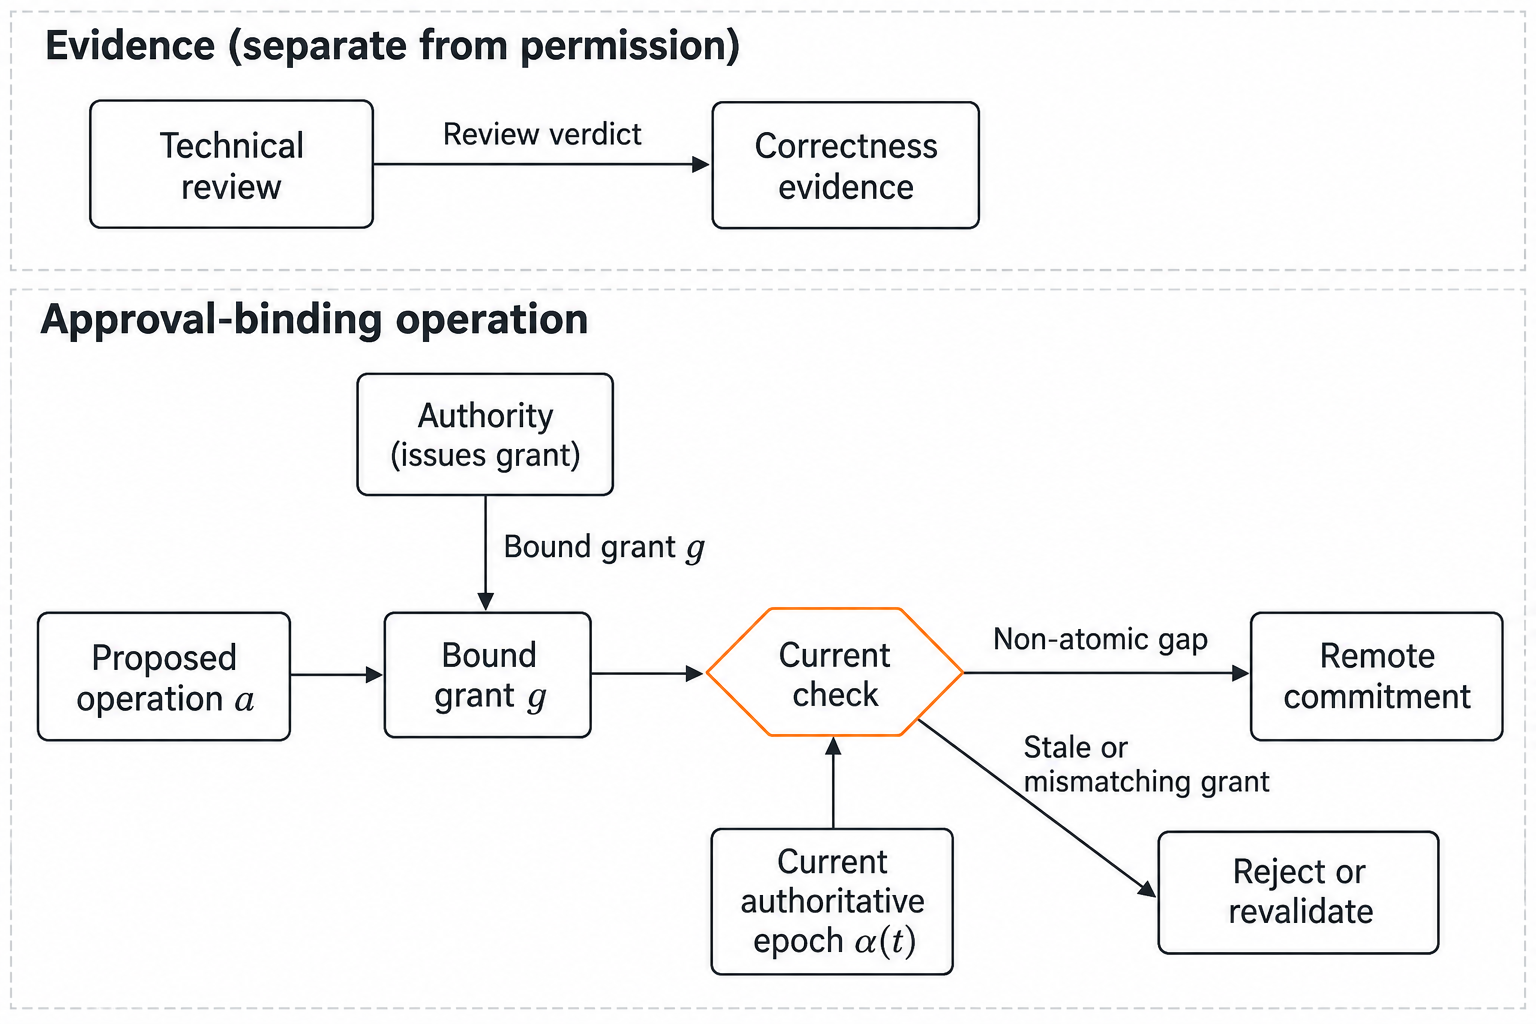
\includegraphics[width=\linewidth]{book/figures/assets/F29review.png}
\caption{Technical review supplies evidence, while an authorized principal grants a specific operation envelope. A current check must bind the principal, arguments, object versions, epoch and expiry. If validation and remote commitment are separate, the service contract must address the remaining race; an earlier approval does not prove current authority or technical correctness.}
\label{fig:C29:overview}
\end{figure}

